\section{Aufbau}
\label{sec:Aufbau}
Der Aufbau für die Biegung eines Stabes bei einseitiger Einspannung \ref{sec:eE}
ist in
Abbildung \ref{fig:abb6} wiedergegeben. Der Versuchsaufbau unterscheidet sich
für die Biegung eines elastischen Stabes bei beidseitiger Auflage
\ref{sec:bA} nur
dahingehend, dass der Stab im Punkt A und B (s. Abb.\ref{fig:abb6}) aufliegt,
anstatt nur in Punkt A.
\begin{figure}
  \centering
  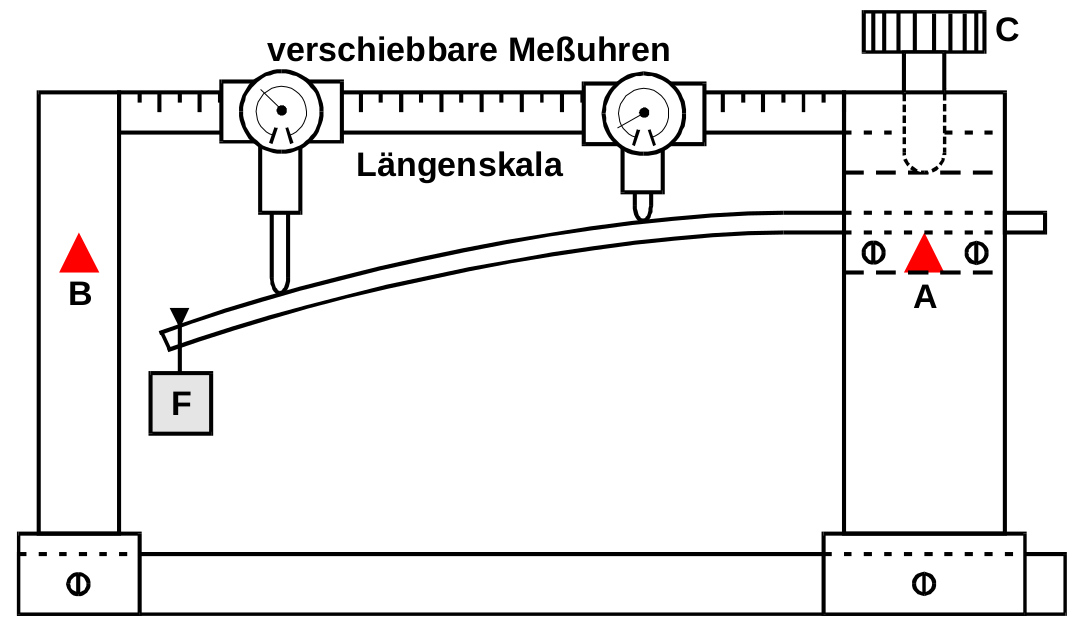
\includegraphics[height = 7cm]{logos/Abb6.png}
  \caption{Darstellung der Versuchsapperatur zur Vermessung elastisch gebogener
  Stäbe aus Quelle \cite{sample}}
  \label{fig:abb6}
\end{figure}
\FloatBarrier
\section{Durchführung}
\label{sec:Durchführung}
\subsection{Biegung eines Stabes bei einseitiger Einspannung}
\label{sec:eE}
Der Stab wird zur erst in die Versuchsapperatur, wie in Abb.\ref{fig:abb6},
mit der Spannvorrichtung C eingespannt. Dann wird eine Messreihe ohne Belastung
aufgenommen. Dabei wird der Stab nur mit einer Tastuhr abgelaufen. Die Werte
werden dann als Referenzwerte $\symup{D_0 (x)}$ genommen. Danach wird eine
Messreihe $\symup{D_M (x)}$
mit Gewichtung aufgenommen. Dabei sollte darauf geachtet werden, dass
die maximale Durchbiegung zwischen 3mm un d 7mm liegt. Für die aufgenommenen
Werte gilt dann:
\begin{equation}
  \symup{D(x) = D_M (x) - D_0 (x)}
  \label{eqn:DM0}
\end{equation}
Dieser Teil des Versuches wurde mit einem rundem und einem eckigen Stab
durchgeführt.
\subsection{Biegung eines Stabes bei beidseitiger Auflage}
\label{sec:bA}
Der Versuchsaufbau wird, wie im Aufbau \ref{sec:Aufbau} geschildert wurde,
aufgebaut. Die Versuchsdurchführung ist hier sehr analog zum Teil\ref{sec:eE}.
Auch hier wird eine Messreihe $\symup{D_0 (x)}$ zur Referenz und eine mit
Gewichtung $\symup{D_M (x)}$ aufgenommen.
Auch hier besteht der Zusammenhang aus Gleichung \eqref{eqn:DM0}.
Der Unterschied besteht darin,
dass nun mit beiden Tastuhren gemessen wird. Eine läuft den Stab von Punkt A bis
zur Mitte und die andere vom Punkt B bis zur Mitte ab. Dieser Teil des Versuches
wurde mit dem rundem Stab von Teil \ref{sec:eE} durchgeführt.
